\documentclass{article}
\usepackage[T1]{fontenc}
\usepackage{lmodern}
\usepackage{graphicx}
\usepackage{amsmath,amssymb}
\usepackage[a4paper,margin=2cm]{geometry}
\usepackage[absolute,overlay]{textpos}
\setlength{\TPHorizModule}{1mm}
\setlength{\TPVertModule}{1mm}
\usepackage[indonesian]{babel}
\usepackage{hyperref}
\setlength{\emergencystretch}{2em}
% unit: Halaman 36

\begin{document}

% === Halaman 36 (llm) ===

\textcolor{red}{\huge Mode CFB-8 bit untuk ukuran blok 64 bit (= 8 byte)}

\vspace{10mm}

(a) Enkripsi

\vspace{10mm}

(b) Dekripsi

% deskripsi: Diagram proses enkripsi Mode CFB-8 bit yang menunjukkan shift register 8-byte, blok enkripsi E dengan kunci K, operasi XOR antara plaintext p_i dan keystream k_i untuk menghasilkan ciphertext c_i.
% bbox normalisasi: [0.1700, 0.2000, 0.4200, 0.8200]
\begin{textblock*}{52.50mm}(35.70mm,59.40mm)
\noindent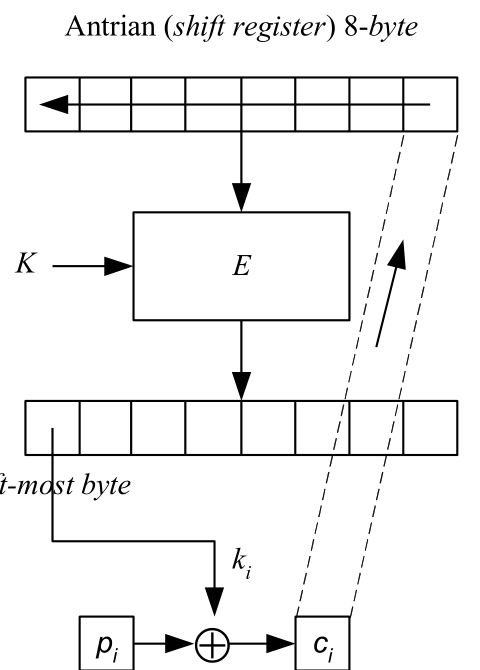
\includegraphics[width=52.50mm,height=184.14mm]{../../images/llm/page_036_img_01.png}%
\end{textblock*}

% deskripsi: Diagram proses dekripsi Mode CFB-8 bit yang menunjukkan shift register 8-byte, blok enkripsi E dengan kunci K, operasi XOR antara ciphertext c_i dan keystream k_i untuk mengembalikan plaintext p_i.
% bbox normalisasi: [0.5600, 0.2000, 0.8400, 0.8200]
\begin{textblock*}{58.80mm}(117.60mm,59.40mm)
\noindent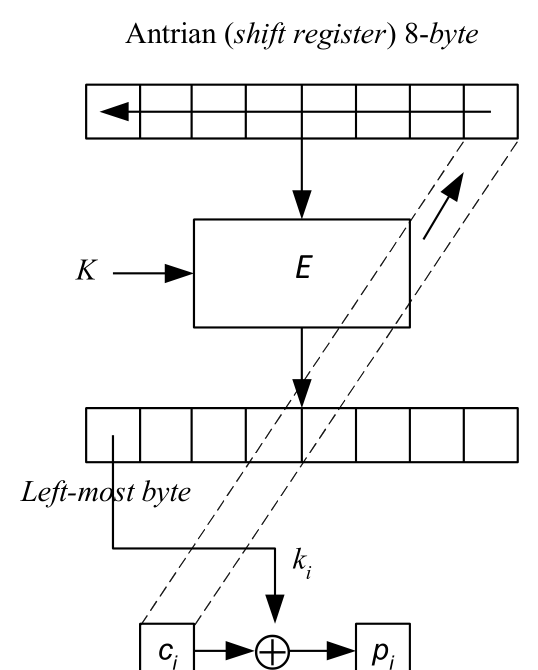
\includegraphics[width=58.80mm,height=184.14mm]{../../images/llm/page_036_img_02.png}%
\end{textblock*}

\end{document}
